%% Poster template using tikzposter
%% see https://ctan.org/pkg/tikzposter  for a manual
%% and https://www.sharelatex.com/templates/53332341910d975953dffdab/v/1/pdf for an example
%% We (see MPIISstyle for authors) added some commands to this to make it even more convinient

%\documentclass[a0paper,portrait]{tikzposter}
\documentclass[a0paper,landscape]{tikzposter} % change paper layout/size
%% If you want a custom paper size use the following. Note that our printer has 106.7cm wide paperroll
%% If you have to print to the margin leave some space to cut it.
%% This would be a large landscape poster
%\documentclass[landscape]{tikzposter}
% \geometry{paperheight=140cm,paperwidth=104cm} % for landscape width and height are swapped






\usepackage{calc}
\usepackage{lipsum}
\usepackage[numbers, sort&compress, square]{natbib}
\usepackage{amsmath}
\usepackage{amssymb}
\usepackage{url}
\usepackage{enumitem}



\usepackage{array}
\usepackage{multirow}
\usepackage{booktabs}

\makeatletter
\newcounter{tablecounter}
\newenvironment{tikztable}[1][]{
  \def \rememberparameter{#1}
  \vspace{10pt}
  \refstepcounter{tablecounter}
  \begin{center}
  }{
    \ifx\rememberparameter\@empty
    \else
    \\[10pt]
    {\small Tab.~\thetablecounter: \rememberparameter}
    \fi
  \end{center}
}
\makeatother

 %if you need algorithm do this:
\usepackage[plain]{algorithm}
 \usepackage{algorithmicx,algpseudocode}
 \usepackage{etoolbox}
 \AtBeginEnvironment{algorithm}{
   \setlength{\columnwidth}{\linewidth}
 }

\algblockdefx{MRepeat}{EndRepeat}{\textbf{repeat}}{}
\algnotext{EndRepeat}

\usepackage[fontscale=0.9]{MPIISposter}
% in addition to the standard latex font sizes we have now also \veryHuge, \VeryHuge, and \VERYHuge
% there is a command
% \fontscale{factor} to scale all fonts

\usetitlestyle{Empty}
%% here you can change the way to boxed look like, see
%% https://bitbucket.org/surmann/tikzposter/downloads/styleguide.pdf
\useblockstyle{Rays}

 %% add your color scheme in this file!


% Cambridge Uni colors from https://www.cam.ac.uk/brand-resources/guidelines/typography-and-colour/rgb-and-websafe-references
\definecolor{camredPantone199}{HTML}{D6083B}
\definecolor{cambluePantone285}{HTML}{0072CF}
\definecolor{camorangePantone158}{HTML}{EA7125}
\definecolor{camgreenPantone369}{HTML}{55A51C}
\definecolor{campurplePantone513}{HTML}{8F2BBC}
\definecolor{camtealPantone7466}{HTML}{00B1C1}
\definecolor{camlredPinkPantone197}{HTML}{EB99A9}
\definecolor{camlbluePantone284}{HTML}{68ACE5}
\definecolor{camlredYellowPantone142}{HTML}{F3BD48}
\definecolor{camlgreenLimePantone583}{HTML}{AAB300}
\definecolor{camlpurplePantone5215}{HTML}{AF95A3}
\definecolor{camltealCambridgeBluePantone557}{HTML}{91B9A4}
\definecolor{camdredPantone1955}{HTML}{901C3B}
\definecolor{camdbluePantone541}{HTML}{003E74}
\definecolor{camdorangePantone718}{HTML}{CB4F00}
\definecolor{camdgreenPantone574}{HTML}{445026}
\definecolor{camdpurplePantone669}{HTML}{422E5D}
\definecolor{camdtealPantone5473}{HTML}{106470}

\definecolorstyle{MPI_rg}{
	\colorlet{colorPrimary}{rgb,255:red,75; green,168; blue,79}
	\colorlet{colorSecondary}{colorPrimary!50!black}
%	\colorlet{colorSecondary}{rgb,255:red,0; green,117; blue,103}
%	\colorlet{colorSecondary}{rgb,255:red,211; green,211; blue,204}
	\colorlet{colorFG}{black}
	\colorlet{colorBG}{white}
	\colorlet{colorFGheader}{white}
	\colorlet{colorBGheader}{black}
}{
	\colorlet{backgroundcolor}{colorBG}
	\colorlet{framecolor}{colorBG!50}
	\colorlet{titlefgcolor}{colorFGheader}
	\colorlet{titlebgcolor}{colorPrimary}
	\colorlet{blocktitlebgcolor}{colorPrimary}
	\colorlet{blocktitlefgcolor}{colorFGheader}
	\colorlet{blockbodybgcolor}{colorBG!10}
	\colorlet{blockbodyfgcolor}{colorFG}
	\colorlet{innerblocktitlebgcolor}{blocktitlebgcolor}
	\colorlet{innerblocktitlefgcolor}{blocktitlefgcolor}
	\colorlet{innerblockbodybgcolor}{blocktitlebgcolor!10}
	\colorlet{innerblockbodyfgcolor}{blockbodyfgcolor}
	\colorlet{notefgcolor}{colorFG}
	\colorlet{notebgcolor}{colorPrimary!20}
	\colorlet{notefrcolor}{colorPrimary}
}

\definecolorstyle{MPI_ei}{
	\colorlet{colorPrimary}{rgb,255:red,255; green,186; blue,77}
	\colorlet{colorSecondary}{rgb,255:red,0; green,117; blue,103}
	\colorlet{colorFG}{black}
	\colorlet{colorBG}{white}
	\colorlet{colorFGheader}{black}
	\colorlet{colorBGheader}{white}
}{
	\colorlet{backgroundcolor}{colorBG}
	\colorlet{framecolor}{colorBG!50}
	\colorlet{titlefgcolor}{colorFGheader}
	\colorlet{titlebgcolor}{colorPrimary}
	\colorlet{blocktitlebgcolor}{colorPrimary}
	\colorlet{blocktitlefgcolor}{colorFGheader}
	\colorlet{blockbodybgcolor}{colorBG!10}
	\colorlet{blockbodyfgcolor}{colorFG}
	\colorlet{innerblocktitlebgcolor}{blocktitlebgcolor}
	\colorlet{innerblocktitlefgcolor}{blocktitlefgcolor}
	\colorlet{innerblockbodybgcolor}{blocktitlebgcolor!10}
	\colorlet{innerblockbodyfgcolor}{blockbodyfgcolor}
	\colorlet{notefgcolor}{colorFG}
	\colorlet{notebgcolor}{colorPrimary!20}
	\colorlet{notefrcolor}{colorPrimary}
}


\definecolorstyle{CAM}{
  \colorlet{colorPrimary}{camdtealPantone5473}
	\colorlet{colorSecondary}{camltealCambridgeBluePantone557}
	\colorlet{colorFG}{black}
	\colorlet{colorBG}{camltealCambridgeBluePantone557!10}
	\colorlet{colorFGheader}{white}
	\colorlet{colorBGheader}{white}
}{
	\colorlet{backgroundcolor}{colorBG}
	\colorlet{framecolor}{colorBG!50}
	\colorlet{titlefgcolor}{colorFGheader}
	\colorlet{titlebgcolor}{colorPrimary}
	\colorlet{blocktitlebgcolor}{colorSecondary}
	\colorlet{blocktitlefgcolor}{colorFGheader}
	\colorlet{blockbodybgcolor}{colorBG!10}
	\colorlet{blockbodyfgcolor}{colorFG}
	\colorlet{innerblocktitlebgcolor}{blocktitlebgcolor}
	\colorlet{innerblocktitlefgcolor}{blocktitlefgcolor}
	\colorlet{innerblockbodybgcolor}{blocktitlebgcolor!10}
	\colorlet{innerblockbodyfgcolor}{blockbodyfgcolor}
	\colorlet{notefgcolor}{colorFG}
	\colorlet{notebgcolor}{colorPrimary!20}
	\colorlet{notefrcolor}{colorPrimary}
}


\usecolorstyle{CAM} % load the respective color scheme
%\usecolorstyle{MPI_ei}

% there is a colorize command that make text appear in the primary color
% you might want to change it if your primary color is very light (here mixed with black 1:1)
%\renewcommand{\colorize}[1]{{\color{blocktitlebgcolor!50!black}\bf #1}}



\newcommand{\xb}{\mathbf{x}}
\newcommand{\Xc}{\mathcal{X}}
\newcommand{\Zc}{{\mathcal{Z}}}
\newcommand{\Mc}{{\mathcal{M}}}
\newcommand{\Bc}{{\mathcal{B}}}
\newcommand{\Ac}{{\mathcal{A}}}
\newcommand{\Pc}{{\mathcal{P}}}
\newcommand{\bb}{{\mathbf{b}}}
\newcommand{\ab}{{\mathbf{a}}}
\newcommand{\mb}{{\mathbf{m}}}
\newcommand{\Mb}{{\mathbf{M}}}
\newcommand{\Pb}{{\mathbf{P}}}
\newcommand{\Hb}{{\mathbf{H}}}
\newcommand{\Ab}{{\mathbf{A}}}
\newcommand{\Rc}{{\mathcal{R}}}
\newcommand{\delb}{{\boldmath{\delta}}}


%
\newcommand{\nodeEmbeddings}[1]{\Hb_{#1}}
\newcommand{\graphEmbeddings}{\mathbf{h_g}}
%\newcommand{\graph}{\mathcal{G}}



\newcommand{\actionLogits}{\textbf{s}} % for nodes

% The model definitions
\newcommand{\electronPath}{\Pc}
\newcommand{\moleculeSet}{\Mc}
\newcommand{\initialAndReactants}{\Mc_0, \Mc_e}

\newcommand{\contextVect}{\bm{c}}
% Then the modules!
\newcommand{\fEmbed}{h_{\Ac}} % for nodes
\newcommand{\fEmbedGraphs}{r} % for nodes
\newcommand{\fEmbedGraphsInclFEmbed}{g}


\newcommand{\fAdd}{f^{\textrm{add}}}
\newcommand{\fRemove}{f^{\textrm{remove}}}
\newcommand{\fInitial}{f^{\textrm{start}}}
\newcommand{\fStop}{f_{\textrm{stop}}}
\newcommand{\fCont}{\fEmbedGraphs^{\textrm{cont}}}
\newcommand{\fReag}{\fEmbedGraphs^{\textrm{reagent}}}

\newcommand{\fContInclEm}{\fEmbedGraphsInclFEmbed^{\textrm{cont}}}
\newcommand{\fReagInclEm}{\fEmbedGraphsInclFEmbed^{\textrm{reagent}}}


\newcommand{\fReagEmbed}{f_{\textrm{reagent}}}
\newcommand{\fModules}{\fEmbed, \fAdd, \fRemove, \fInitial,\fStop, \fReagEmbed}
\newcommand{\fui}{f_\textrm{gate}}
\newcommand{\fuj}{f_\textrm{up}}
\newcommand{\fuk}{f_\textrm{down}}
\newcommand{\fum}{f_m}

\newcommand{\actionProb}[2][]{ p(a_{#2} \mid \moleculeSet_{\electronPath_{0:#2-1}^{#1}}, a^{#1}_{#2-1}, #2)}
\newcommand{\continueProb}[2]{p(s_{#1}' \mid \moleculeSet_{#2}) }


% Our model
\newcommand{\ourModel}{\textsc{ELECTRO}}
\newcommand{\ourModelIR}{\textsc{ELECTRO-LITE}}
\newcommand{\ourModelR}{\textsc{ELECTRO}}


\newcommand{\neigh}[1]{\mathcal{N}_{e#1}}









\newcommand{\PosterDepartment}{}
\newcommand{\PosterTitle}{ A Generative Model For Electron Paths}
\newcommand{\PosterAuthor}{  John Bradshaw\textsuperscript{1,2},
  Matt J. Kusner\textsuperscript{3,4},
Brooks Paige\textsuperscript{1,4},
 Marwin H. S. Segler\textsuperscript{5}, 
 Jos\'e Miguel Hern\'andez-Lobato\textsuperscript{1,4,6}}
 \newcommand{\PosterAff}{
  \textsuperscript{1}University of Cambridge,
  \textsuperscript{2}MPI for Intelligent Systems,
\textsuperscript{3}University of Oxford,
\textsuperscript{4}The Alan Turing Institute, 
\textsuperscript{5}BenevolentAI,
\textsuperscript{6}Microsoft Research Cambridge.
  }

\renewcommand{\PosterFooter}{
arXiv:1805.10970   \hfill jab255@cam.ac.uk, mkusner@turing.ac.uk, bpaige@turing.ac.uk, marwin.segler@benevolent.ai, jmh233@cam.ac.uk
}



\definecolor{reactionAdd}{HTML}{1bb41f}
\definecolor{reactionRemove}{HTML}{ff3226}


\renewcommand{\familydefault}{\sfdefault}
\title{\PosterTitle}
\author{\PosterAuthor}

\settitle{
  \s{1.5}
  \begin{center}
    \color{titlefgcolor}
    {\VERYHuge \bfseries \PosterTitle\\[0.3em]}
    {\huge \PosterAuthor\\[.5em]}
    {\large \PosterAff}
  \end{center}
  \null
}

\begin{document}
\maketitle[titletotopverticalspace=0cm,titletoblockverticalspace=1.5cm]
%% decide about black or white Minerva
%% BTW: the Minerva looking into the poster is nicer than if she looks out, so on the left
%\addlogoleft{logos/Max-Planck-Gesellschaft-white}
% \addlogoleft{logos/Max-Planck-Gesellschaft-black}

%% you can add another logo and shift it inwards if you want
%\addlogoright[5cm]{yourlogo}

\posterfooter


\begin{columns}
  \column{0.36}

 % \specialblock{Overview}{


 %   \colorize{\bf Our goal:}
 %   Provide an easy to use poster template with:
 %   \begin{itemize}
 %   \item easy to change color schemes
 %   \item proper title area scaling
 %   \item arbitrary paper size
 %   \end{itemize}
 %   \s{.5}
 % }

  \block{Aim: predict reaction outcomes through predicting the movement of electrons (the reaction mechanism)}{
    \begin{cols}
    \col{.50}
    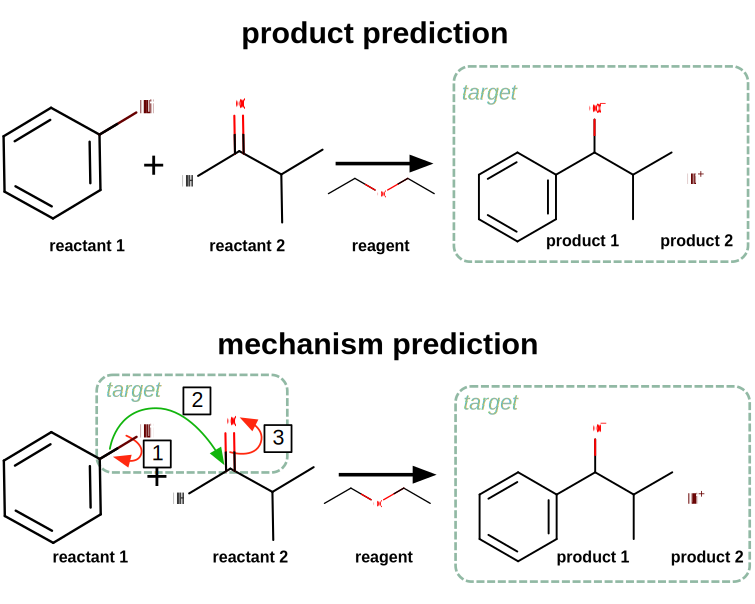
\includegraphics[width=\linewidth]{imgs/inkscape_img_edits/reaction_diagram.pdf}
    \col{.02}
    \col{.48}
      \begin{itemize}
        \item Reactions involve the step wise movement of electrons along the atoms: this \textcolor{reactionRemove}{\bf removes} and \textcolor{reactionAdd}{\bf adds} bonds.
        \item Recent approaches of ML applied to reaction prediction \citep{jin2017predicting,schwaller2017found} have focused on product prediction.
        \item We also want to know how the reactants formed the products.
        \item Therefore, we instead approach the problem from the angle
          of mechanism prediction: this provides \colorize{interpretability}, takes advantage of the \colorize{sparsity} of reactions, and naturally \colorize{incorporates the constraints of chemistry} (eg balanced atom counts).
        \item We model reactions exhibiting linear electron flow (LEF) topology, the most common occurring of reactions \citep{herges1994coarctate}.
      \end{itemize}
    \end{cols}


  }



  % \block{Commands}{
  %   \colorize{\bf Some nifty features:}
  %   Here are some of the commands we added to make life easier:
  %  \begin{enumerate} % verb// does not work inside of block
  %  \item {\tt fontscale} argument allows to scale all fonts (easy to refit poster)
  %  \item {\tt \textbackslash{}colorize\{test\}} makes text \colorize{colored} (automatically fitting to box color)
  %  \item {\tt \textbackslash{}s\{X\}} create a vertical space in units of em (relative to fontsize)
  %  \item {\tt cols} environment creating a multicolumn inside a box
  %    with {\tt \textbackslash{}col\{0.5\}} creating a new column with relative size
  %  \item {\tt \textbackslash{}ig[relsize]\{img\}} short for includegraphics with relative width to column (default 1.0)
  %  \end{enumerate}%

  %  \innerblock{interesting}{

  %    Normal text or \colorize{colorized text}
  %  }

  %  \s{1} % add some spacing
  %  \innerblock{}{
  %    box without header
  %  }

  %  \s{1}
  %  placing pics works great with cols environment (like in beamer with columns)
  %  \s{1}

  %  \begin{cols}
  %    \col{.4}
  %    \ig{logos/Max-Planck-Gesellschaft-black}
  %    \col{.2} \centering
  %    some text in between
  %    \col{.4}
  %    \ig{logos/Max-Planck-Gesellschaft-black}

  %  \end{cols}
  %}

  % COLUMN 2
  % ---------------------------------------------------------------------------
  \column{0.64}

  \block{Our model, \textsc{ELECTRO}, uses graph neural networks to parameterize the probability of each kind of action}{

  \begin{cols}
  \col{0.27}

  Reactions exhibiting LEF topology have a single electron path consisting of alternating \textcolor{reactionRemove}{\bf remove} and \textcolor{reactionAdd}{\bf add} bond steps.
  
    \begin{algorithm}[H]
    %\caption{}
    \begin{algorithmic}[1]
      \State Select \textcolor{camorangePantone158}{\bf starting} atom A using 
      \textcolor{camorangePantone158}{\bf $p_\theta^{\mathrm{start}}(a \mid \moleculeSet_0, \moleculeSet_e)$}
      %\triangleq \mbox{softmax}\Big[f^{\mathrm{start}}\big(h_{\Ac}(\moleculeSet_0), g^\mathrm{reagent}(\Mc_e)\big)\Big]$
      \MRepeat
      \State Select atom B bonded to A using \textcolor{reactionRemove}{\bf $p_\theta^{\mathrm{remove}}(a_t | \moleculeSet_t, a_{t-1})$}
        and \textcolor{reactionRemove}{\bf remove} 2 electrons from bond B-A.
        \State Decide whether to \textcolor{campurplePantone513}{\bf continue} using  \textcolor{campurplePantone513}{\bf $p_\theta^{\textrm{cont}}(c_{t+1} \mid \moleculeSet_{t+1})$}.
        \State Select new atom A using \textcolor{reactionAdd}{\bf $p_\theta^{\mathrm{add}}(a_t | \moleculeSet_t, a_{t-1})$} and \textcolor{reactionAdd}{\bf add} bond B-A.
        \State Decide whether to  \textcolor{campurplePantone513}{\bf continue} using  \textcolor{campurplePantone513}{\bf $p_\theta^{\textrm{cont}}(c_{t+1} \mid \moleculeSet_{t+1})$}.
      \EndRepeat
    \end{algorithmic}
    \end{algorithm}
  \col{0.02}
  \col{0.72}
  { \raggedright
    \includegraphics[width=\linewidth]{imgs/reaction_model_color_coded.pdf}
  }


  \end{cols}

  }


\end{columns}

\block{We can extract these approximate electron paths from large scale reaction databases (such as USPTO \citep{USPTO_bitbucket}) for training \textsc{ELECTRO}}
{
  Reaction datasets often store reactions as atom-mapped SMILES strings, e.g.{ \tt  \small [CH3:10][N:11]1[CH2:12][CH2:13][C:14](=[O:17])[CH2:15][CH2:16]1.[F:1][c:2]1[c:3]([CH2:4][Cl:5])[cH:6][cH:7][cH:8][cH:9]1  $>>$
  [F:1][c:2]1[c:3]([CH2:4][C:14]2([OH:17])[CH2:13][CH2:12][N:11]([CH3:10])[CH2:16][CH2:15]2)[cH:6][cH:7][cH:8][cH:9]1}

  From this we want to extract the reactants, the reagents, the products, and an approximate electron path for training our model.

\includegraphics[width=\linewidth]{imgs/inkscape_img_edits/extract_path.pdf}
}

\begin{columns}
  \column{0.4}

  \block{Assessing \textsc{ELECTRO} for mechanism prediction}{
    \begin{cols}
      \col{0.36}
        \includegraphics[height=9cm]{imgs/main_text_input.pdf}
      \col{0.04}
      \col{0.64}

      \begin{tikztable}[Results when using \textsc{ELECTRO} for \emph{mechanism prediction}.
      Here a prediction is correct if the atom mapped action sequences predicted by our model match exactly those extracted from the USPTO dataset.
      \ourModelIR \; is an ablation study for which we hide the reagents from our model.]
        \begin{tabular}{lllll}
          \toprule
          & \multicolumn{4}{c}{Accuracies (\%)}                   \\
          \cmidrule(r){2-5}
          Model Name & Top-1 & Top-2 & Top-3 & Top-5 \\
          \midrule
          \ourModelIR &  70.3 &  82.8 & 87.7 & 92.2    \\
          \ourModelR  &  77.8 &  89.2 & 92.4 & 94.7    \\
          \bottomrule
        \end{tabular}
       % \caption{Results when using \textsc{ELECTRO} for \emph{mechanism prediction}.
        %Here a prediction is correct if the atom mapped action sequences predicted by our model match exactly those extracted from the USPTO dataset.}
      \end{tikztable}

    \end{cols}
    \vspace{1cm}

    \begin{cols}
      \col{0.5}
      \includegraphics[height=7cm]{imgs/reaction3.pdf}
      \col{0.5}
      \includegraphics[height=7cm]{imgs/reaction7.pdf}

    \end{cols}



}

  \column{0.35}

  \block{Assessing \textsc{ELECTRO} for product prediction}{
    \begin{cols}
    \col{0.36}

    Assessing only for predicting mechanisms means that predicting the correct product in an alternative way is labeled as incorrect.
    This may not be what we always want, eg with \colorize{symmetry}:
    \includegraphics[width=0.8\linewidth]{imgs/possible1.pdf}

    \includegraphics[width=0.8\linewidth]{imgs/possible2.pdf}

    

    \col{0.06}
    \col{0.6}
    \begin{center}  $\therefore$ We also evaluate \textsc{ELECTRO} for product prediction.
    \end{center}

\vfill

    \begin{tikztable}[Results for \emph{product prediction}.
      For the baselines we compare against models trained (a) on the 
      full USPTO training set (marked FTS) and only tested on our subset of LEF reactions,
      and (b) those that are also trained on the same subset as our model.
      \ourModelIR \; is an ablation study for which we hide the reagents from our model.]
  \begin{tabular}{lllll}
    \toprule
    & \multicolumn{4}{c}{Accuracies (\%)}                   \\
    \cmidrule(r){2-5}
    Model Name & Top-1 & Top-2 & Top-3 & Top-5 \\
    \midrule
    WLDN FTS \citep{jin2017predicting} & 84.0  & 89.2 &  91.1 & 92.3 \\
    WLDN \citep{jin2017predicting} & 83.1 & 89.3 & 91.5 & 92.7 \\
    Seq2Seq FTS \citep{schwaller2017found} & 81.7 & 86.8 & 88.4 & 89.8 \\
    Seq2Seq \citep{schwaller2017found} & 82.6 & 87.3 & 88.8 & 90.1\\
    \bottomrule \toprule
    \ourModelIR &  78.2 & 87.7 & 91.5 & 94.4   \\
    \ourModelR  &  {\bf 87.0} & {\bf 92.6} & {\bf 94.5} & {\bf 95.9}    \\
    \bottomrule
  \end{tabular}
  \end{tikztable}



    \end{cols}



  }

  \column{0.25}
%% References
  \block{}{
    % use bibtex here
     \nocite*  % use this to force all entries in the bibfile to go here
    % \bibliography{mybib}
    % or the manual entries (can be copied from .bbl files in case you have used bibtex on a document)
    \setlength{\bibsep}{.2em}
    \begin{thebibliography}{1}

      \bibitem{jin2017predicting}
     Jin, Wengong, Connor Coley, Regina Barzilay, and Tommi Jaakkola.
     \newblock Predicting Organic Reaction Outcomes with Weisfeiler-Lehman Network.
    %\newblock Advances in Neural Information Processing Systems 30, 2017.
    \newblock NeurIPS, 2017.


    \bibitem{schwaller2017found}
    Schwaller, Philippe, Theophile Gaudin, David Lanyi, Costas Bekas, and Teodoro Laino.
    \newblock “Found in Translation”: predicting outcomes of complex organic chemistry reactions using neural sequence-to-sequence models.
    \newblock Chem. Sci., 2018.

    \bibitem{herges1994coarctate}
     Herges, Rainer.
     \newblock Coarctate Transition States: The Discovery of a Reaction Principle.
      \newblock Journal of chemical information and computer sciences, 1994.

    \bibitem{NIPS2011_4356}
    Kayala, Matthew A., and Pierre F. Baldi.
    \newblock A Machine Learning Approach to Predict Chemical Reactions.
    %\newblock  Advances in Neural Information Processing Systems 24, 2011.
    \newblock   NeurIPS, 2011.

    \bibitem{USPTO_bitbucket}
    Lowe, Daniel Mark.
    \newblock Extraction of chemical structures and reactions from the literature.
    \newblock PhD diss., University of Cambridge, 2012.


    \end{thebibliography}
  }

\end{columns}

\end{document}
